\section{Evaluation Metrics}

\subsection{Content Preservation} \label{content-preservation-metric}

\subsection{Cycle Loss}

Cycle loss is not a good metric because while transferring from $X$ to $Y$, and back to $X'$, the variable $Y$ is not observable and if the neural network function is accidentally fitted to transform the content domain, this metric will not be able to tell the difference between an over-fit model and a good model.


\section{Experiment Results}

We conducted experiments on an Amazon product review data-set, following \cite{fu2017style}. It contains 131072, 2048, 32768 sentences for train, validation, and test, respectively, each sampling accompanied by binary sentiment labels.

\subsection{Disentangling Latent Space}

We first analyze how the style (sentiment) and content of the latent space are disentangled. We train a logistic classifier based on different latent spaces, and show results in Table~\ref{tab:classification}.

We see that the 128-dimensional content vector is not discriminative for style. It achieves an accuracy of 0.57, slightly better than random/majority guess. However, the 8-dimensional style vector $\bm s$, despite its low dimensionality, achieves significantly higher style classification accuracy. When combining content and style vectors, we achieve no further improvement. These results verify the effectiveness of our disentangling approach, because the style space does contain style information, whereas the content space doesn't.


\begin{table}
	\centering
	\begin{tabular}{| l | r |}
		\hline
		Random/Majority guess           & 0.5000          \\ \hline
		Content latent space  ($\bm c$) & 0.5690          \\
		Style latent space ($\bm s$)    & \textbf{0.7817} \\
		Combined ($[\bm s;\bm c]$)      & 0.7815          \\
		\hline
	\end{tabular}
	\caption{Style classification accuracy.}
	\label{tab:classification}
\end{table}

\begin{figure}
	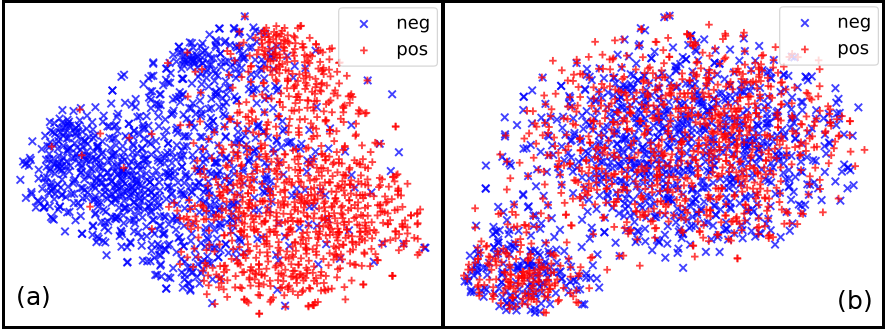
\includegraphics[width=\linewidth]{images/tsne-style-and-content}
	\caption{t-SNE plots of (a) style and (b) content spaces.}
	\label{fig:tsne}
\end{figure}


The latent space can be visualized with t-SNE plots~\cite{maaten2008visualizing} in Figure~\ref{fig:tsne}. As expected, sentences with different sentiments can be nicely separated in the style space (LHS), but are highly mixed in the content space (RHS).


\subsection{Style-Transfer Sentence Generation}

We apply the disentangled latent space to a style-transfer sentence generation task, where the goal is to generate a sentence with different sentiment (style). We followed \cite{fu2017style} and used two metrics: (1) For style transfer, we train a style classifier and predict the accuracy of the generated sentences. While the style classifier itself may not be perfect, it provides a quantitative way of evaluating the strength of style transfer. (2) For the content-preservation score, we compute a sentence embedding by min, max, and average pooling of word embeddings; then a cosine similarity is computed to evaluate how close two sentences are in meaning. Here, sentiment words from a stop list \cite{hu2004mining} are removed.

We compare our approach with state-of-the-art previous work in Table~\ref{tab:comparison-previous}. We re-conducted the experiments with their publicly available code on our data splits.
Results show that, our approach achieves a comparable content-preservation score with previous work, but a significantly better style-transfer score, showing that our disentangled latent space can be used for better style-transfer sentence generation.

Table~\ref{tab:ablation-results} presents the results of an ablation test. We see that both adversarial loss and reconstruction loss play a role in the strength of style transfer, and that they can be combined to further improve performance.

Some examples of style-transfer sentence generation are illustrated in Table~\ref{tab:transfer-samples}. We see that, with the empirically estimated style vector, we can flexibly control the sentiment of generated sentences.

\begin{table}[!t]
	\centering
	\begin{tabular}{| l | r | r | }
		\hline
		\textbf{Model}                       & \textbf{Style Transfer} & \textbf{Content Preservation} \\
		\hline
		\hline
		Cross-alignment \cite{shen2017style} & 0.4609                  & 0.8830                        \\
		\hline
		Sentiment embed. \cite{fu2017style}  & 0.4009                  & 0.9246                        \\
		\hline
		Ours                                 & 0.7708                  & 0.8958                        \\
		\hline
	\end{tabular}
	\caption{Comparison with previous approaches.}
	\label{tab:comparison-previous}
\end{table}

\begin{table}[!t]
	\centering
	\begin{tabular}{| l | r | r |}
		\hline
		\textbf{Training Loss}                          & \textbf{Style Transfer} & \textbf{Content Preservation} \\
		\hline
		\hline
		$J_\text{rec}$                                  & 0.5053                  & 0.9103                        \\
		\hline
		$J_\text{rec}$, $J_\text{adv}$                  & 0.5901                  & 0.9121                        \\
		\hline
		$J_\text{rec}$, $J_\text{mult}$                 & 0.6445                  & 0.9053                        \\
		\hline
		$J_\text{rec}$, $J_\text{adv}$, $J_\text{mult}$ & 0.7708                  & 0.8958                        \\
		\hline
	\end{tabular}
	\caption{Ablation test.}
	\label{tab:ablation-results}
\end{table}

\begin{table}[!t]
	\centering
	\begin{tabular}{| p{0.45\linewidth} | p{0.45\linewidth} |}
		\hline
		\textbf{{Original}}                                                        & \textbf{Transferred (Positive $\rightarrow$ Negative)}                    \\
		\hline
		\hline
		i bought this cuisipro mister to replace my old mister last june-(number)  & i bought this a couple of times and was disappointed in this product      \\
		\hline
		quality is good, recevied in time and works as expected.                   & quality is good but i am returning it                                     \\
		\hline
		all in all, i am very happy with this headset.                             & all in all i was expecting a good product                                 \\
		\hline
		\hline
		\textbf{{Original}}                                                        & \textbf{Transferred (Negative $\rightarrow$ Positive)}                    \\
		\hline
		\hline
		i sent it back and requested a refund, and never got the refund.           & i sent it back and gave it a try and it works great                       \\
		\hline
		so i tried just one (number) piece each n still the same results.          & so i bought the two sizes and the other ones are great                    \\
		\hline
		i am going to buy a replacement and wish i had sent this back for a refund & i am going to go through the same time and i have been using it for years \\
		\hline
	\end{tabular}
	\caption{Examples of style-transfer generation.}
	\label{tab:transfer-samples}
\end{table}
